% Created 2024-10-18 Fri 20:26
% Intended LaTeX compiler: pdflatex
\documentclass[11pt]{article}
\usepackage[utf8]{inputenc}
\usepackage[T1]{fontenc}
\usepackage{graphicx}
\usepackage{longtable}
\usepackage{wrapfig}
\usepackage{rotating}
\usepackage[normalem]{ulem}
\usepackage{amsmath}
\usepackage{amssymb}
\usepackage{capt-of}
\usepackage{hyperref}
\usepackage{parskip,darkmode}
\enabledarkmode
\usepackage{algorithm,algpseudocode}
\usepackage{tikz}
\usetikzlibrary{trees, arrows.meta}
\author{Arnav Gupta}
\date{\today}
\title{Decision Trees And Training Strategies}
\hypersetup{
 pdfauthor={Arnav Gupta},
 pdftitle={Decision Trees And Training Strategies},
 pdfkeywords={},
 pdfsubject={},
 pdfcreator={Emacs 29.4 (Org mode 9.7.11)}, 
 pdflang={English}}
\begin{document}

\maketitle
\tableofcontents

\section{Decision Trees}
\label{sec:org212fe35}
Technique for supervised learning from discrete data:
\begin{itemize}
\item representation is a decision tree
\item bias towards simple decision tree
\item search through space of decision trees, from simple to complex
\end{itemize}

For each \textbf{decision tree}:
\begin{itemize}
\item \textbf{nodes}: input attributes/features
\item \textbf{branches}: labeled with input feature values (can have multiple feature values on one branch)
\item \textbf{leaves}: predictions for target features (point estimates)
\end{itemize}

\begin{center}
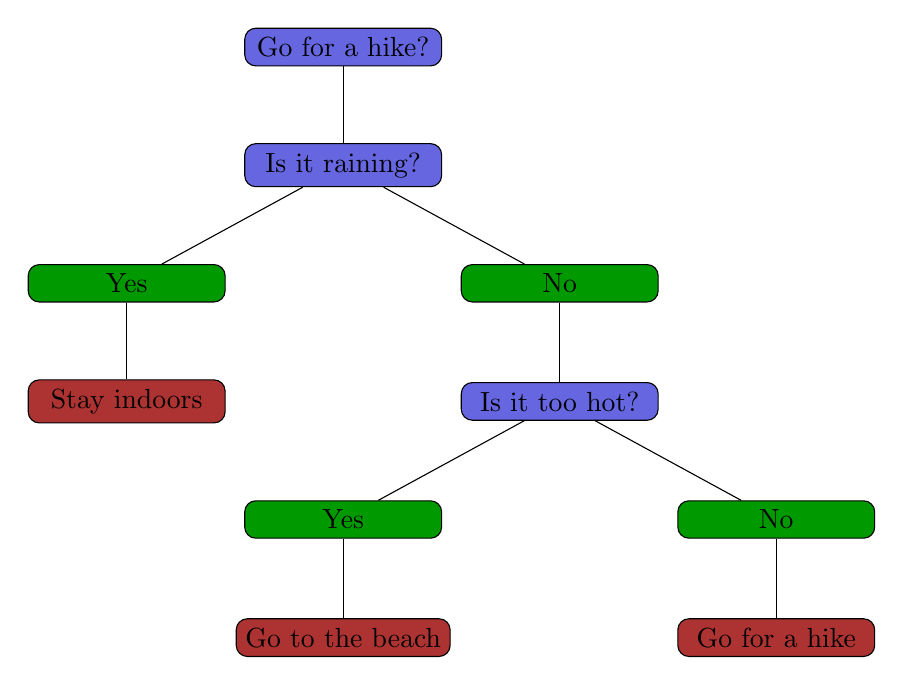
\begin{tikzpicture}[every node/.style={draw, rectangle, rounded corners, align=center, minimum width=2.5cm},
                    level distance=1.5cm,
                    sibling distance=5.5cm] % Increase sibling distance
    % Root node
        \node[fill=blue!80!black!60] {Go for a hike?}
        child { node[fill=blue!80!black!60] {Is it raining?}
            child { node[fill=green!60!black!100] {Yes}
                child { node[fill=red!60!black!80] {Stay indoors} } % Leaf
            }
            child { node[fill=green!60!black!100] {No}
                child { node[fill=blue!80!black!60] {Is it too hot?}
                    child { node[fill=green!60!black!100] {Yes}
                        child { node[fill=red!60!black!80] {Go to the beach} } % Leaf
                    }
                    child { node[fill=green!60!black!100] {No}
                        child { node[fill=red!60!black!80] {Go for a hike} } % Leaf
                    }
                }
            }
        };
\end{tikzpicture}
\end{center}

To learn a decision tree:
\begin{enumerate}
\item split training data based some criteria (bias)
\item recursively solve sub-problems
\end{enumerate}

Criteria for good decision trees: small, good classification (low error on training data), good generalization (low error on test data).

\begin{algorithm}
\caption{Decision Tree Learner}
\begin{algorithmic}[1]
\Procedure{DecisionTreeLearner}{X, Y, E}
    \If{stopping criteria is met}
        \State \Return pointEstimate(Y, E)
    \Else
        \State select input feature \( X_i \in X \)
        \For{each value \( x_i \) of \( X_i \)}
            \State \( E_i \gets \) all examples in \( E \) where \( X_i = x_i \)
            \State \( T_i \gets \text{DecisionTreeLearner}(X \setminus \{X_i\}, Y, E_i) \)
        \EndFor
        \State \Return \( \langle X_i, T_1, \ldots, T_N \rangle \)
    \EndIf
\EndProcedure
\end{algorithmic}
\end{algorithm}

\begin{algorithm}
\caption{Classify Example}
\begin{algorithmic}[1]
\Procedure{ClassifyExample}{e, X, Y, DT}
    \State \( S \gets DT \)
    \While{S is an internal node of the form \( \langle X_i, T_1, \ldots, T_N \rangle \)}
        \State \( j \gets X_i(e) \)
        \State \( S \gets T_j \)
    \EndWhile
    \State \Return S
\EndProcedure
\end{algorithmic}
\end{algorithm}
\subsection{Stopping Criteria}
\label{sec:org1ed547c}
Related to the final return value, depends on what must be done.

Possible stopping criteria:
\begin{itemize}
\item no more features
\item performance on training data good enough
\end{itemize}
\subsection{Feature Selection}
\label{sec:orgd81a515}
Choose sequence of features that result in smallest tree.

In practice, split based on what gives best performance.

Heuristics for best performing feature:
\begin{itemize}
\item most even split
\item max info gain
\item GINI index
\end{itemize}
\section{Information Theory}
\label{sec:orgd8f4b3c}
\(n\) bits can distinguish \(2^{n}\) items, but can do better with probabilities.

In general, need \(-\log_{2} P(x)\) bits to encode \(x\).
Each symbol requires on average
$$
-P(x)\log_{2} P(x) \text{ bits}
$$

To transmit an entire sequence distributed according to \(P(x)\),
$$
\sum_{x} -P(x)\log_{2} P(x) \text{ bits}
$$
bits of info per symbol are needed on average, which is the \textbf{info content} or \textbf{entropy} of the sequence.
\subsection{Information Gain}
\label{sec:org3e81235}
Given a set \(E\) of \(N\) training examples, if the number of examples with output feature \(Y = y_{i}\)
is \(N_{i}\), then
$$
P(Y = y_{i}) = P(y_{i}) = \frac{N_{i}}{N}
$$
is the point estimate.

The total info content for \(E\) is
$$
I(E) = - \sum_{y_{i} \in Y} P(y_{i}) \log( P(y_{i}) )
$$
After splitting \(E\) into \(E_{1}\) and \(E_{2}\) based on input feature \(X_{i}\), the information
content is
$$
I(E_{split}) = \frac{N_{1}}{N} I(E_{1}) + \frac{N_{2}}{N} I(E_{2})
$$
so the desirable \(X_{i}\) is the one that maximizes \textbf{info gain}:
$$
I(E) - I(E_{split}) = - \sum_{y \in Y} P(y) \log P(y) + \sum_{x \in X, y \in Y} \log \frac{P(x,y)}{P(x)}
\ge -\log \left( \sum_{x \in X, y \in Y} P(x, y) \frac{P(x)P(y)}{P(x, y)} \right)
$$

Info gain is the reduction in uncertainty about the output feature \(T\) given the value
of a certain input feature \(X\).

\textbf{Jensen's inequality}: for a convex function \(f(x)\), \(E[f(x)] \ge f(E[x])\).
\section{Training Strategies}
\label{sec:org09be2ee}
\subsection{Final Return Value}
\label{sec:orgc3fe50c}
Point estimate (prediction of target features) of \(Y\) over all examples.

A point estimate could be mean, median, mode, or
$$
P(Y = y_{i}) = \frac{N_{i}}{N}
$$
\subsection{Priority Queue}
\label{sec:org5c1dab0}
Sort leaves using a priority queue ranked by how much info can be gained with the best feature at that
leaf.
Always expand the leaf at the top of the queue.

\begin{algorithm}
\caption{Decision Tree Learner}
\begin{algorithmic}[1]
\Procedure{DecisionTreeLearner}{X, Y, E}
    \State \( DT \gets \text{pointEstimate}(Y, E) \) \Comment{initial decision tree}
    \State \( \{ X', \Delta I \} \gets \text{best feature and Information Gain value for } E \)
    \State \( PQ \gets \{ (DT, E, X', \Delta I) \} \) \Comment{priority queue of leaves ranked by \( \Delta I \)}
    \While{stopping criteria is not met}
        \State \( \{ S_\ell, E_\ell, X_\ell, \Delta I_\ell \} \gets \text{leaf at the head of } PQ \)
        \For{each value \( x_i \) of \( X_\ell \)}
            \State \( E_i \gets \) all examples in \( E_\ell \) where \( X_\ell = x_i \)
            \State \( \{ X_j, \Delta I_j \} \gets \text{best feature and value for } E_i \)
            \State \( T_i \gets \text{pointEstimate}(Y, E_i) \)
            \State insert \( \{ T_i, E_i, X_j, \Delta I_j \} \) \text{ into } \( PQ \text{ according to } \Delta I_j \)
        \EndFor
        \State \( S_\ell \gets \langle X_\ell, T_1, \ldots, T_N \rangle \)
    \EndWhile
    \State \Return \( DT \)
\EndProcedure
\end{algorithmic}
\end{algorithm}
\subsection{Overfitting}
\label{sec:org3dece28}
When there is not enough data, the decision tree does not generalize to test data.

Methods to avoid overfitting:
\begin{itemize}
\item \textbf{regularization}: prefer small decision trees, so add a complexity penalty to stopping criteria
\item \textbf{pseudocounts}: add data based on prior knowledge
\item \textbf{cross validation}
\end{itemize}

\begin{center}
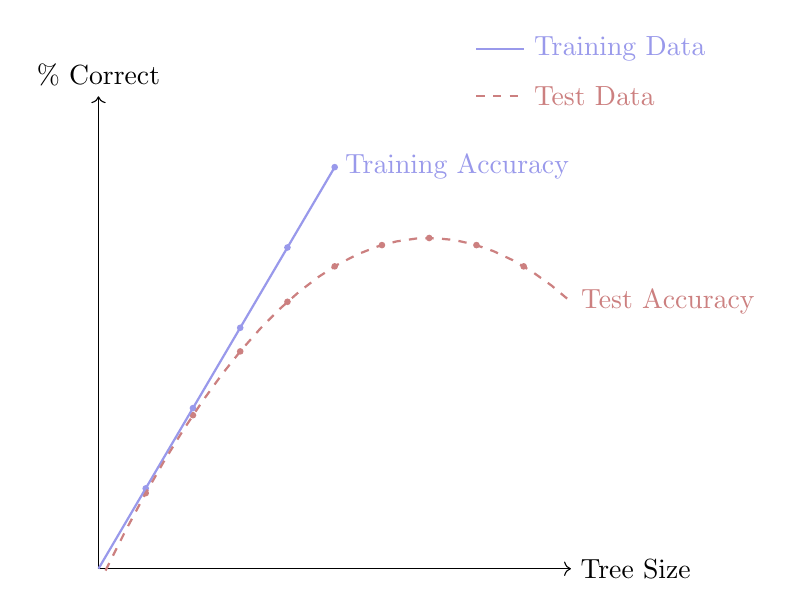
\begin{tikzpicture}[scale=0.6] % Adjust scale for better visibility
    % Axes
    \draw[->] (0,0) -- (10,0) node[right] {Tree Size};
    \draw[->] (0,0) -- (0,10) node[above] {\% Correct};

    % Training data points (increasing accuracy with tree size)
    \foreach \x in {1,2,...,5} {
        \fill[blue!80!black!40] (\x, {1.7 * \x}) circle (2pt); % Training accuracy increases
    }

    % Test data points (accuracy increases then decreases)
    \foreach \x in {1,2,...,9} {
        \fill[red!60!black!50] (\x, {7 - 0.15 * (\x - 7)^2}) circle (2pt); % Test accuracy rises then falls
    }

    % Training line
    \draw[blue!80!black!40, thick] plot[domain=0:5] (\x, {1.7 * \x}) node[right] {Training Accuracy};

    % Test line (parabolic decline)
    \draw[red!60!black!50, thick, dashed] plot[domain=0.15:10] (\x, {7 - 0.15 * (\x - 7)^2}) node[right] {Test Accuracy};

    % Legend
    \draw[blue!80!black!40, thick] (8, 11) -- (9, 11) node[right] {Training Data};
    \draw[red!60!black!50, thick, dashed] (8, 10) -- (9, 10) node[right] {Test Data};
\end{tikzpicture}
\end{center}

Test set errors are caused by:
\begin{itemize}
\item \textbf{bias}: error due to the algorithm finding an imperfect model
\begin{itemize}
\item \textbf{representation bias}: model too simple
\item \textbf{search bias}: not enough search
\end{itemize}
\item \textbf{variance}: error due to lack of data
\item \textbf{noise}: error due to data depending on features not modeled or because process generating
data is stochastic
\item \textbf{bias-variance trade-off}
\begin{itemize}
\item complicated model, not enough data
\item simple model, lots of data
\end{itemize}
\end{itemize}

\textbf{Capacity}: ability of a model to fit a wide variety of functions (inverse of bias)

\textbf{Cross Validation}:
\begin{itemize}
\item split training data into training and validation set
\item use validation set as fake test set
\item optimize decision maker to perform well on validation set
\item repeat with different validation sets
\end{itemize}
\end{document}
